\chapter{Detailed Design}

\section{Interface Design}

This section deals with how this software interacts with people, hardware and other software.

\subsection{The Users}
The webApp interacts with users using UI components designed on React. The users can enter text in the text boxes for various purposes such as searching, sending information regarding free softwares and proprietary softwares and obtaining license information.

\subsection{Other softwares}
Various modules have been implemented and imported throughout the project to enable different software components to interact with each other. Modules such as ‘express’ and ‘mongoose’ have been used to connect api endpoints with implemented functions and connect to the database respectively. The back-end implemented on nodejs is integrated with the front end react components using RESTful API.

\section{Data Structures and Algorithms}
This section deals with various functions implemented along with their purposes and the data structures used.

\subsection{\texttt{createProprietarySoftware}}
This function is used to create a new proprietary software by taking information from the user-end. This function will only be accessible when the user searches for a proprietary software and its not available already. Then if the user wishes to request for the proprietary software, he can submit the request consisting of the name of the proprietary software along with other details such as a short description regarding the software along with a tag that will be used while searching for  alternatives for this software.

A json object will be used to send data regarding this software using key-value pairs to the back-end to process and add this data to the database.

A input validation happens at the database level and the user is prompted with a input error if the format of the input does not match the required specification.

\subsection{\texttt{getTopAlternatives}}
This function is used when the user wants to know the trending alternatives with the maximum upvotes. This function returns an array of json objects containing the properties of the top 10 alternatives sorted in descending order of their upvotes. The user does not need to specify any input for this function as it directly fetches data from the database. 

In case the number of documents in the alternatives section of the database is less than 10, all the alternatives are returned in descending order. However, if there’s no data in the alternative softwares section this function returns 0, which can be further used to display relevant error messages to the user.

\subsection{\texttt{createFreeSoftware}}
Similar to the addProprietarySoftware, this function is used to add alternative software for a specific proprietary software. The user needs to specify the name, short description, license fields of the alternative software. The handle field of the alternative json object is set using the tags field of the proprietary software for which the alternative is being suggested.

A json object will be used to send data regarding this software using key-value pairs to the back-end to process and add this data to the database.

A input validation happens at the database level and the user is prompted with a input error if the format of the input does not match the required specification.

\subsection{\texttt{getAllFreeSoftwares}}
This function fetches all the free softwares from the database along with their short descriptions, upvotes and license. It will be used in case the user wishes to see all the alternatives which are available on the website and this returned value can be used for performing various other manipulations on the retrieved data which can be used to meet the needs of some other functions which can be implemented in future.
An array of json objects will be returned by this function containing properties like name and a short description, license and upvotes of the software. 

No input validation is required as the function does not take any input. However, if there are no free softwares present in the database, the function returns a suitable error message.


\subsection{\texttt{checkLicense}}
This function takes a pattern as parameter which will be used to match it to the names of the alternatives in the database and returns an array of objects containing the license information of all the matching results. The matching is performed by treating the pattern as a regExp ignoring the case.

If the pattern doesn’t match any alternative in the database, a suitable error message is returned. 

\subsection{\texttt{getProprietarySoftwares}}
This function takes a pattern as parameter which will be used to match it to the names of the proprietary softwares in the database and returns an array of objects containing the name, short description and tags information of all the matching results. The matching is performed by treating the pattern as a regExp ignoring the case.

If the pattern doesn’t match any proprietary software in the database, a suitable error message is returned. 


\subsection{\texttt{getAllProprietarySoftwares}}
This function fetches all the proprietary softwares from the database along with their short descriptions. It will be used in case the user wishes to see all the proprietary softwares which are available on the website and this returned value can be used for performing various other manipulations on the retrieved data which can be used to meet the needs of some other functions which can be implemented in future.
An array of json objects will be returned by this function containing properties like name and a short description, license and upvotes of the software. 

No input validation is required as the function does not take any input. However, if there are no free softwares present in the database, the function returns a suitable error message.


\subsection{\texttt{getAlternatives}}
This function takes in the id of a proprietary software in the database and returns an array of json objects of alternatives to this particular proprietary software (corresponding to the id). The handle of the alternative is searched for in the tags field of the proprietary softwares. If found, the alternative is concluded to be an alternative of this proprietary software and is added to the array of results which will be returned by this function.

If no proprietary software is found for the specified id, the function will return a suitable error message.

\subsection{\texttt{increaseUpvotes}}
This function simply increases the upvotes property of the alternative software specified by its id which will be specified as a parameter to this function.

In case no alternative is found corresponding to the passed id, a suitable error message is returned by this function.

\subsection{\texttt{decreaseUpvotes}}
This function simply decreases the upvotes property of the alternative software specified by its id which will be specified as a parameter to this function.

In case no alternative is found corresponding to the passed id, a suitable error message is returned by this function.


\section{UML Diagrams and Discussions}

\begin{center}
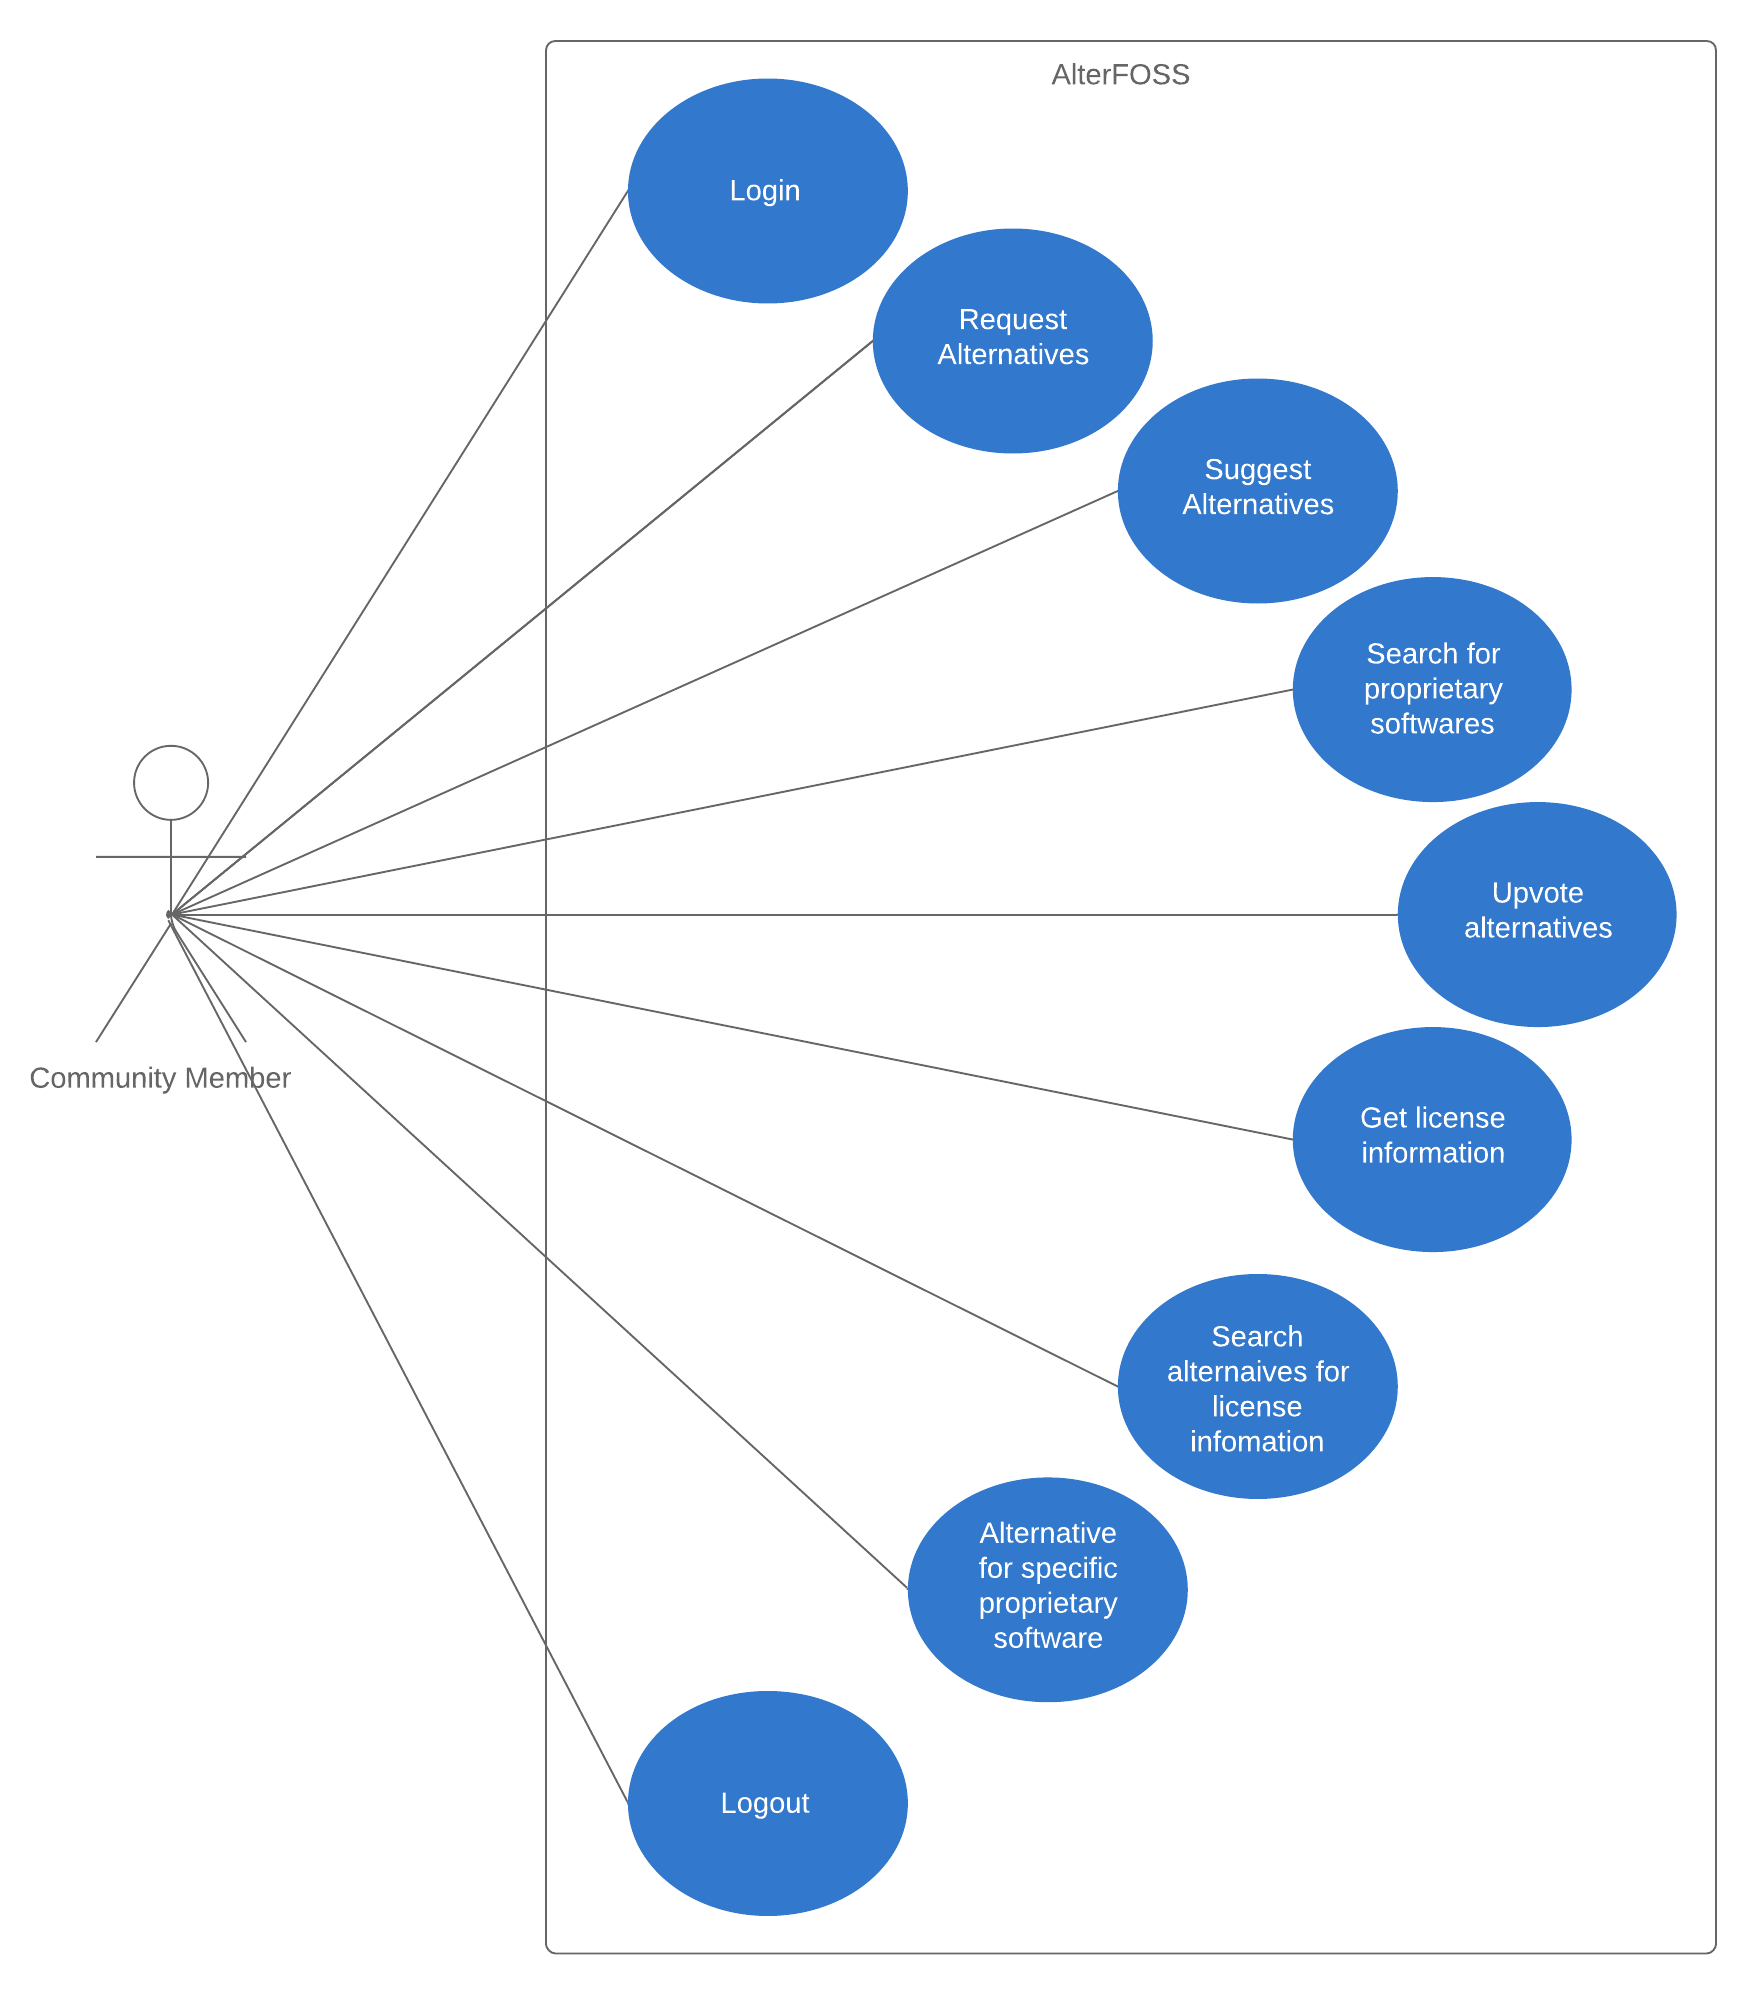
\includegraphics[scale=1]{images/uml_user.png} 
\captionof{figure}{User-case diagram of AlterFoss}
\end{center}

As shown above in the use-case diagram, this entire platform will be community driven. Once logged in, the regular community members will have the facilities to post new proprietary softwares to request for its alternatives, suggest alternatives for already posted requests (proprietary softwares) as well as get already posted alternatives. The users can search for proprietary softwares and upvote specific alternatives. The users can also retrieve the top 10 voted alternatives and check the license information of all posted alternatives. Also, searching and license checking do not require logging in.

\pagebreak

\section{Data Source/Database used and formats}

This section deals with the database used and the format in which the data is stored in the database.

\subsection{Details on Database}
The database used for this project is \textbf{MongoDB} which is a free and open-source cross-platform document-oriented database program. MongoDB uses JSON-like documents with schemas and is classified as a NOSQL database. It is published under a combination of the GNU Affero General Public License and the Apache License.

\subsection{Data format/schemas}
There are majorly 3 entities used in the project:
\begin{itemize}
\item proprietarysoftware
\item freesoftwares
\item usercredentials
\end{itemize}

Each of these entities are being stored as mongodb documents. The detailed structure/format of all these entities is as follows:


\subsubsection{Proprietarysoftware}
This schema contains the following fields :

\begin{description}
\item[name : ]
A string used to store the name of the proprietary software. This field is required and can’t be set to empty.

\item[shortDescription : ]
A string used to store a single line description for the proprietary software. This field is also required.

\item[tags : ]
An array of strings used to characterize the proprietary software. These strings can be used to find suitable alternatives for this proprietary software. This field also has a validator function set to make sure that the user specifies at least one tag for every proprietary software.

\item[requestedBy : ] 
A string used to store the name of the user who posted this proprietary software to request for its alternatives. If no value is specified for this field during the creation of the proprietary software, “anonymous” is taken as the default value.

\end{description}

\medskip

\subsubsection{Freesoftware}
This schema contains the following fields :

\begin{description}

\item[name : ]
A string used to store the name of the alternative. This field is required and can’t be set to empty.

\item[shortDescription : ] 
A string used to store a single line description for the alternative. This field is also required. 

\item[upVotes : ]
An integer to store the number of upvotes of the alternative. Can be used by the community to evaluate the quality of the alternative. Initialized to zero initially.

\item[downVotes : ]
An integer to store the number of downvotes of the alternative. Can be used by the community to evaluate the quality of the alternative. This property is currently not being used but will be considered for future functionality. Initialized to zero initially.

\item[handle : ]
A string which will characterize the alternative. This property will be used to find which proprietary software this alternative is fit for. This field is probably the most important one as this is the one which will pair it with its proprietary counterpart.

\item[license : ]
 A string which stores the name of the license under which this software was published. This field is required thus it cannot be empty.
 
\item[SuggestedBy : ]
 A string which stores the name of the user who suggested this alternative. If no value is specified for this field during the creation of the proprietary software, \textsl{“anonymous”} is taken as the default value.

\end{description}

\medskip

\subsubsection{Usercredentials}

This schema contains the following fields :

\begin{description}

\item[firstName : ]
A string used to store the first name of the user. This field is required and can be a combination of alphabets with a maximum length of 50. This specification is validated by using a regExp for this field.

\item[lastName : ]
A string to store the last name of the user. This field is required and can be a combination of alphabets with a maximum length of 50. This specification is validated by using a regExp for this field.

\item[gender : ]
A string to store the gender of the user, which can be one of the three enumerated values: male, female, or something-else.
userName: A string to store the username of the user. This can be a combination of alphanumeric characters and - with a minimum length of 3 and a maximum length of 30 as specified by the regExp validating this field. This field must be unique for every user.

\item[password : ]
A string to store the hash of the user’s password. This too is a required field.

\item[email : ]
A string to store the e-mail of the user. This field is required and must be unique for every user. This field is also validated by a regular expression and can have a maximum length of 255.

\item[hasUpvoted : ]
An array to store the ids of the alternatives for which the user has upvoted. This can be used to verify that the user cannot upvote the software for which he has already upvoted.
\end{description}


































